\begin{Example}[haireye3]{Hair color and eye color}

The program below reads the hair and eye color data into the \Dset\
\pname{HAIREYE}, and calls the \proc{CORRESP}.  This example illustrates
the use of \PROC{PLOT} and the Annotate facility with \PROC{GPLOT} to
produce a labeled display of the correspondence analysis solution.
To input a contingency table in the CORRESP step, the hair colors
(columns) are specified as the variables in the \stmt{VAR}{CORRESP}, and
the eye colors (rows) are indicated as the ID variable.
%% \inclsas{corresp3)
%% input: /users/faculty/friendly/sasuser/catdata/corresp3.sas
%% last modified: 28-Jul-98 17:26
\begin{listing}
data haireye;
   input  EYE $ BLACK BROWN RED BLOND ;
datalines;
         Brown    68   119    26     7    
         Blue     20    84    17    94    
         Hazel    15    54    14    10    
         Green     5    29    14    16    
;
proc corresp data=haireye outc=coord short;
    var black brown red blond;
    id eye;
proc print data=coord;
   var _type_ eye dim1 dim2 quality;
\end{listing}

\ixd{hair-eye color}

The printed output from the \proc{CORRESP} is shown in
\outref{out:corresp3.1}.  The
section labeled ``Inertia and Chi-Square Decomposition'' indicates that over 98\% of the
Pearson
\(\chi^2\) for association is accounted for by two dimensions, with
most of that attributed to the first dimension.

\begin{Output}[htb]
\caption{Hair-eye data, \PROC{CORRESP} printed output}\label{out:corresp3.1}
\small
\verbatiminput{ch5/out/corresp3.1}
\end{Output}
\ixd{hair-eye color}

A plot of the row and column points can be constructed from the \pname{OUTC=}
\Dset\ \pname{COORD} requested in the \PROC{CORRESP} step.  The variables of
interest in this example are shown in \outref{out:corresp3.2}.  Note that row and
column points are distinguished by the variable \verb|_TYPE_|.
The labels for the points are stored in the \pname{id} variable,
\pname{eye} in this example.

\begin{Output}[htb]
\caption{Hair-eye data, OUTC=coord \Dset}\label{out:corresp3.2}
\small
\verbatiminput{ch5/out/corresp3.2}
\end{Output}
\ixd{hair-eye color}

The interpretation of the correspondence analysis results is
facilitated by a \emph{labeled} plot of the row and column points.
As of Version 6.08, points can be labeled in \PROC{PLOT}.  The
statements below produce a labeled plot.  The plot should be
scaled so that the number of data units/inch are the same for both
dimensions.  Otherwise, the distances (and angles) in this plot would not be
represented accurately.  In \PROC{PLOT}, this is done with the
\opt{VTOH}{PLOT}, which specifies the aspect ratio (vertical to
horizontal) of your printer, together with the \pname{HAXIS} and
\pname{VAXIS} options.

The \opt{VTOH}{PLOT} tries to equate distances between tick marks,  so you should
specify the same tick increment (e.g., \pname{HAXIS=BY xx}, \pname{VAXIS=BY xx}) for both axes.
For example, this \PROC{PLOT} step produces the
printer plot shown in \outref{out:corresp3.3}.
\ix{equating axes}

\begin{listing}
proc plot data-coord vtoh=2;
   plot dim2 * dim1 = '*'$ eye / box haxis=by .1 vaxis=by .1;
run;
\end{listing}

\begin{Output}[htb]
\caption{Labeled printer plot for the hair color, eye color \CA\ solution}\label{out:corresp3.3}
{\footnotesize
\begin{verbatim}
                 Plot of DIM2*DIM1$EYE.  Symbol used is '*'.
     -+----+----+----+----+----+----+----+----+----+----+----+----+----+----+-
DIM2 |                                                                       |
     |                                                                       |
 0.4 +                                                                       +
     |                                 * Green                               |
 0.3 +                   * RED                                               +
     |                                                                       |
 0.2 +                                                                       +
     |              * Hazel                                                  |
 0.1 +                                                                       +
     |                  * BROWN                                              |
 0.0 +                                                                       +
     |                                                             BLOND *   |
-0.1 +* Brown                                             * Blue             +
     |                                                                       |
-0.2 +* BLACK                                                                +
     |                                                                       |
-0.3 +                                                                       +
     |                                                                       |
     -+----+----+----+----+----+----+----+----+----+----+----+----+----+----+-
    -0.5 -0.4 -0.3 -0.2 -0.1  0.0  0.1  0.2  0.3  0.4  0.5  0.6  0.7  0.8  0.9
                                       DIM1
\end{verbatim}
}
\end{Output}
\ixd{hair-eye color}

A labeled high-resolution display of the correspondence analysis
solution (\figref{fig:corresp3}) is constructed with \PROC{GPLOT},
using a DATA step to produce an \ADS\ \pname{LABELS} from
the \pname{COORD} \Dset.  In the \PROC{GPLOT} step, axes are equated with
the AXIS statements: AXIS1 specifies a length and range which are
both twice that in the AXIS2 statement, so that the ratio of data
units to plot units is the same in both dimensions.
That is, the \pname{LENGTH} options are set so that
\ix{AXIS@\texttt{AXIS} statement!LENGTH@\texttt{LENGTH} option}
\ix{axes!equating}
\begin{equation*}
 \frac{ x_{\mbox{max}} - x_{\mbox{min}} } {  x_{\mbox{length}}} =
 \frac{ y_{\mbox{max}} - y_{\mbox{min}} } {  y_{\mbox{length}}}
 \period
\end{equation*}
Alternatively, you may use the \macro{EQUATE}
from the \SASSAMP\,
(see the \STUG\, Chapter 19, Example 3) 
which calculates the
desired lengths from the coordinates, or simply scale the aspect ratio
of the plot by using the options \texttt{HSIZE=} and \texttt{VSIZE=}
of the \texttt{GOPTIONS} statement.%
\footnote{The \texttt{HSIZE=} and \texttt{VSIZE=} options control the
entire plot size, including axis labels, titles and footnotes, so
setting these options, while easier, is less exact than setting the axis lengths.
}
The \macro{CORRESP}, illustrated in the next section, uses a version of the
\macro{EQUATE} (\macref{mac:equate}) modified to scale the plot automatically.
%% \inclsas{corresp3)
%% \input{corres3b} %% level: 3
%% input: /users/faculty/friendly/sasuser/catdata/corresp3.sas
%% last modified: 28-Jul-98 17:26
\begin{listing}
data label;
   set coord;
   xsys='2'; ysys='2';
   x = dim1; y = dim2;
   text = eye;
   size = 1.3;
   function='LABEL';
   if _type_='VAR' then color='RED  '; else color='BLUE'; 
data key;
    xsys='5'; ysys='5';
    length text $12;
    x = 25; y = 77;
    size = 1.4;
    color = 'BLUE ';
    function = 'LABEL   '; text = '* Eye color ' ; output;
    x = 55;
    color = 'RED  ';
    function = 'LABEL   '; text = '* HAIR COLOR' ; output;
data label;
    set key label;
proc gplot data=coord;
   plot dim2 * dim1
        / anno=label frame
          href=0 vref=0 lvref=3 lhref=3
          vaxis=axis2 haxis=axis1
          vminor=1 hminor=1;
   axis1 length=6 in  order=(-1. to 1. by .5)
         label=(h=1.5          'Dimension 1');
   axis2 length=3 in  order=(-.5 to .5 by .5)
         label=(h=1.5 a=90 r=0 'Dimension 2');
   symbol v=none;
run;
\end{listing}

\ixd{hair-eye color}

\begin{figure}[htb]
  \centering
  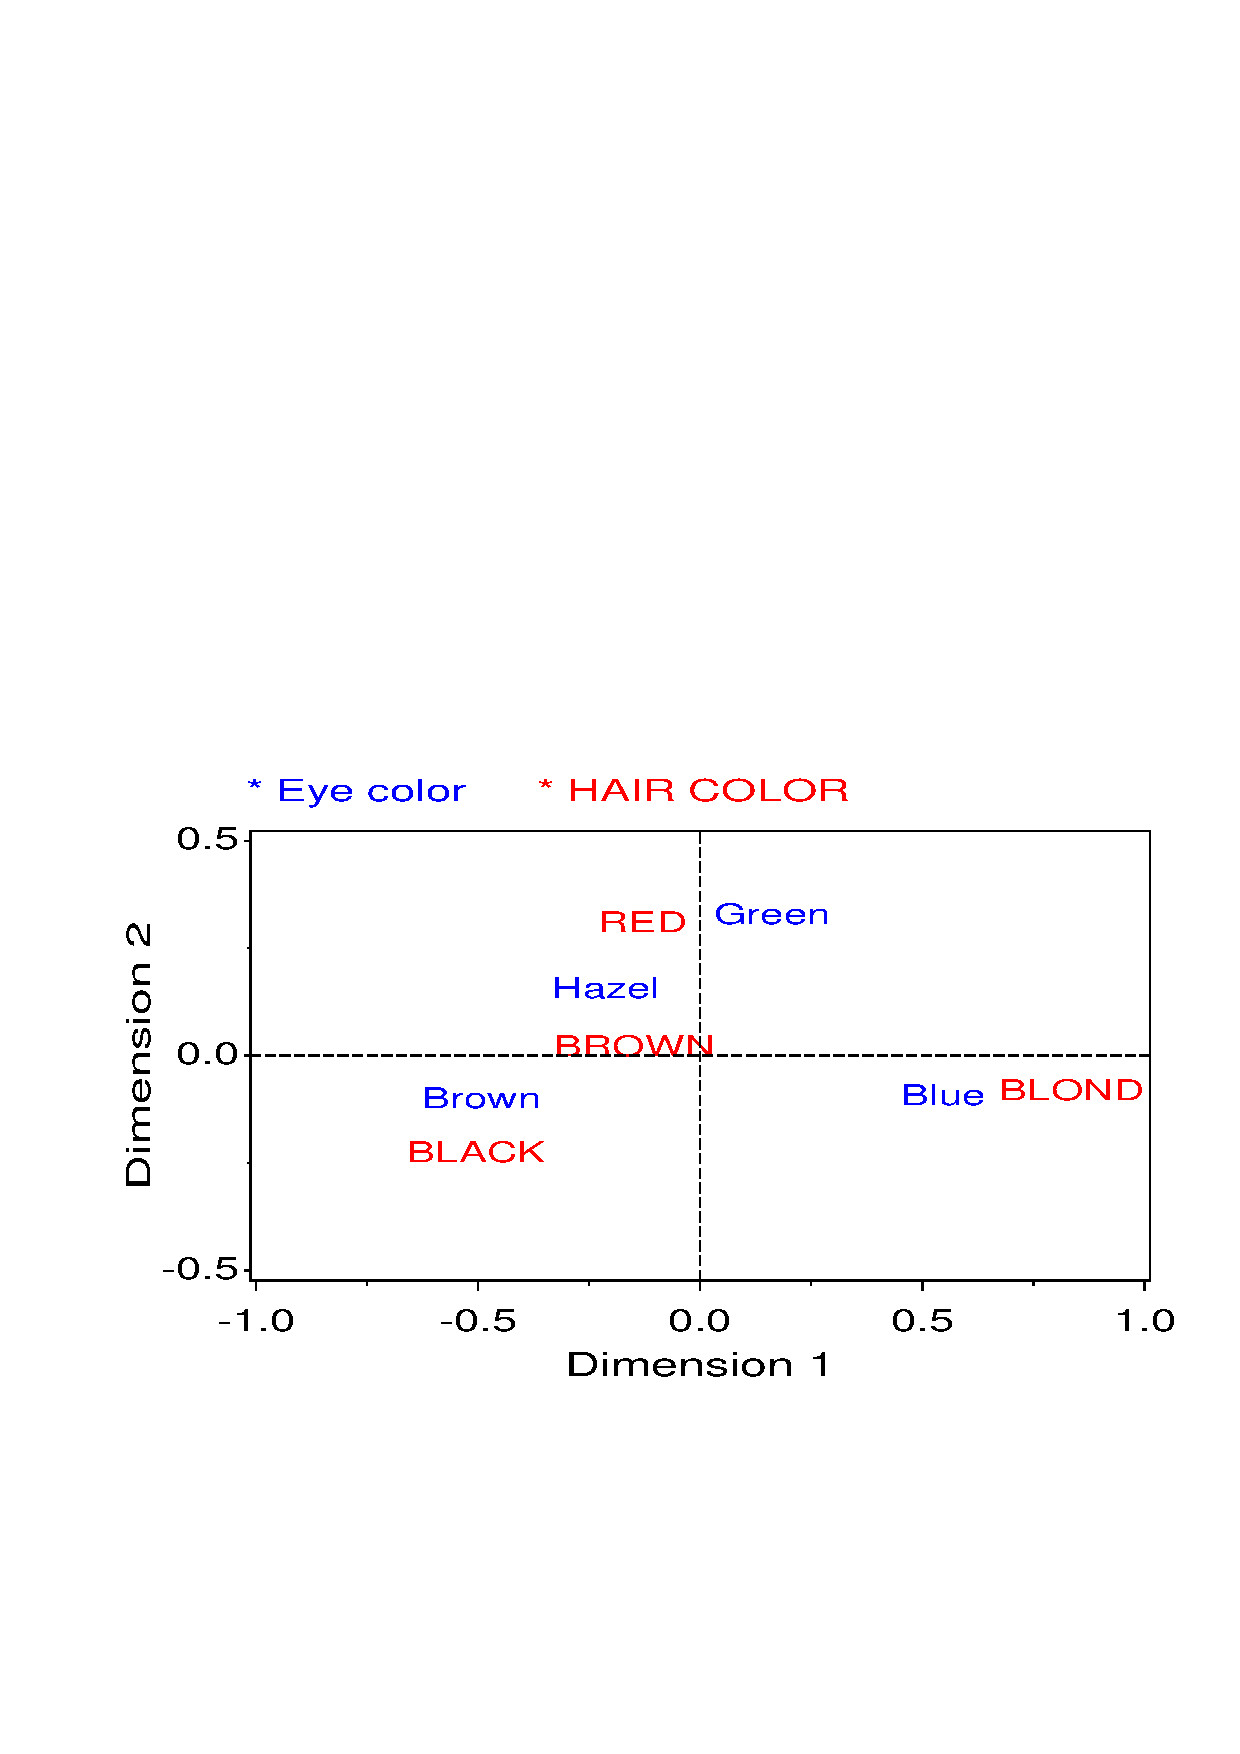
\includegraphics[scale=.7,clip=true]{ch5/fig/corresp3}
  \caption{Correspondence analysis solution for
Hair color, Eye color data}\label{fig:corresp3}
\end{figure}
\ixd{hair-eye color}
\end{Example}
